\ylDisplay{Kiil} % Ülesande nimi
{Valter Kiisk} % Autor
{lõppvoor} % Voor
{2007} % Aasta
{G 3} % Ülesande nr.
{2} % Raskustase
{
% Teema: Geomeetriline-optika
\ifStatement
Laserkiire teele asetatakse enam-vähem risti õhuke klaasplaat (klaasi murdumisnäitaja $n = \num{1,5}$). Selle tulemusena nihkub $L = \SI{2}{m}$ kaugusel ekraanil olev laserkiire kujutis $d = \SI{5}{mm}$ võrra. Järeldatakse, et plaat on kergelt kiilukujuline. Leidke selle kiilu tipunurk $\alpha$. 

\emph{Vihje}. Väikeste nurkade $\varphi$ puhul $\sin \varphi \approx \tan \varphi \approx \varphi$.
\fi


\ifHint
laserkiire kõrvalekaldenurk on leitav Snelli seaduse ja kiilu geomeetria rakendamisest.
\fi


\ifSolution
Kõik nurgad on tähistatud järgneval joonisel. $\alpha$ on meelevaldne (kuigi $\alpha \ll 1$). $\beta = \alpha /n$. $\gamma = \beta - \epsilon$. $\delta = n\gamma = \alpha - n\epsilon$. Kiire kõrvalekaldenurk
\[
\phi=(\alpha-\beta)-(\delta-\gamma)=(\alpha-\delta)+(\gamma-\beta)=n \epsilon-\epsilon=\epsilon(n-1).
\]
Teades, et $\phi = \SI{5}{mm}/\SI{2}{m} = \SI{0.0025}{rad}$, saame
\[
\epsilon=\frac{\phi}{n-1}=\SI{0,005}{rad}=\SI{0,29}{\degree}.
\]

\begin{center}
	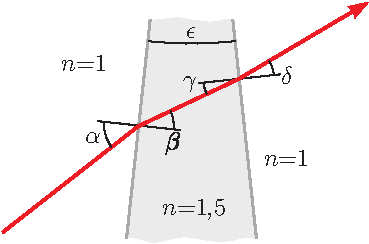
\includegraphics[width=0.7\textwidth]{2007-v3g-03-yl}
\end{center}
\fi
}